\documentclass[11pt,a4paper]{report}
\usepackage[textwidth=37em,vmargin=30mm]{geometry}
\usepackage{calc,xunicode,amsmath,amssymb,paralist,enumitem,tabu,booktabs,datetime2,xeCJK,xeCJKfntef,listings}
\usepackage{tocloft,fancyhdr,tcolorbox,xcolor,graphicx,eso-pic,xltxtra,xelatexemoji}

\newcommand{\envyear}[0]{2025}
\newcommand{\envdatestr}[0]{2025-10-03}
\newcommand{\envfinaldir}[0]{webdb/2025/20251003/final}

\usepackage[hidelinks]{hyperref}
\hypersetup{
    colorlinks=false,
    pdfpagemode=FullScreen,
    pdftitle={Web Digest - \envdatestr}
}

\setlength{\cftbeforechapskip}{10pt}
\renewcommand{\cftchapfont}{\rmfamily\bfseries\large\raggedright}
\setlength{\cftbeforesecskip}{2pt}
\renewcommand{\cftsecfont}{\sffamily\small\raggedright}

\setdefaultleftmargin{2em}{2em}{1em}{1em}{1em}{1em}

\usepackage{xeCJK,xeCJKfntef}
\xeCJKsetup{PunctStyle=plain,RubberPunctSkip=false,CJKglue=\strut\hskip 0pt plus 0.1em minus 0.05em,CJKecglue=\strut\hskip 0.22em plus 0.2em}
\XeTeXlinebreaklocale "zh"
\XeTeXlinebreakskip = 0pt


\setmainfont{Brygada 1918}
\setromanfont{Brygada 1918}
\setsansfont{IBM Plex Sans}
\setmonofont{JetBrains Mono NL}
\setCJKmainfont{Noto Serif CJK SC}
\setCJKromanfont{Noto Serif CJK SC}
\setCJKsansfont{Noto Sans CJK SC}
\setCJKmonofont{Noto Sans CJK SC}

\setlength{\parindent}{0pt}
\setlength{\parskip}{8pt}
\linespread{1.15}

\lstset{
	basicstyle=\ttfamily\footnotesize,
	numbersep=5pt,
	backgroundcolor=\color{black!5},
	showspaces=false,
	showstringspaces=false,
	showtabs=false,
	tabsize=2,
	captionpos=b,
	breaklines=true,
	breakatwhitespace=true,
	breakautoindent=true,
	linewidth=\textwidth
}






\newcommand{\coverpic}[2]{
    % argv: itemurl, authorname
    Cover photo by #2~~(\href{#1}{#1})
}
\newcommand{\makeheader}[0]{
    \begin{titlepage}
        % \newgeometry{hmargin=15mm,tmargin=21mm,bmargin=12mm}
        \begin{center}
            
            \rmfamily\scshape
            \fontspec{BaskervilleF}
            \fontspec{Old Standard}
            \fontsize{59pt}{70pt}\selectfont
            WEB\hfill DIGEST
            
            \vfill
            % \vskip 30pt
            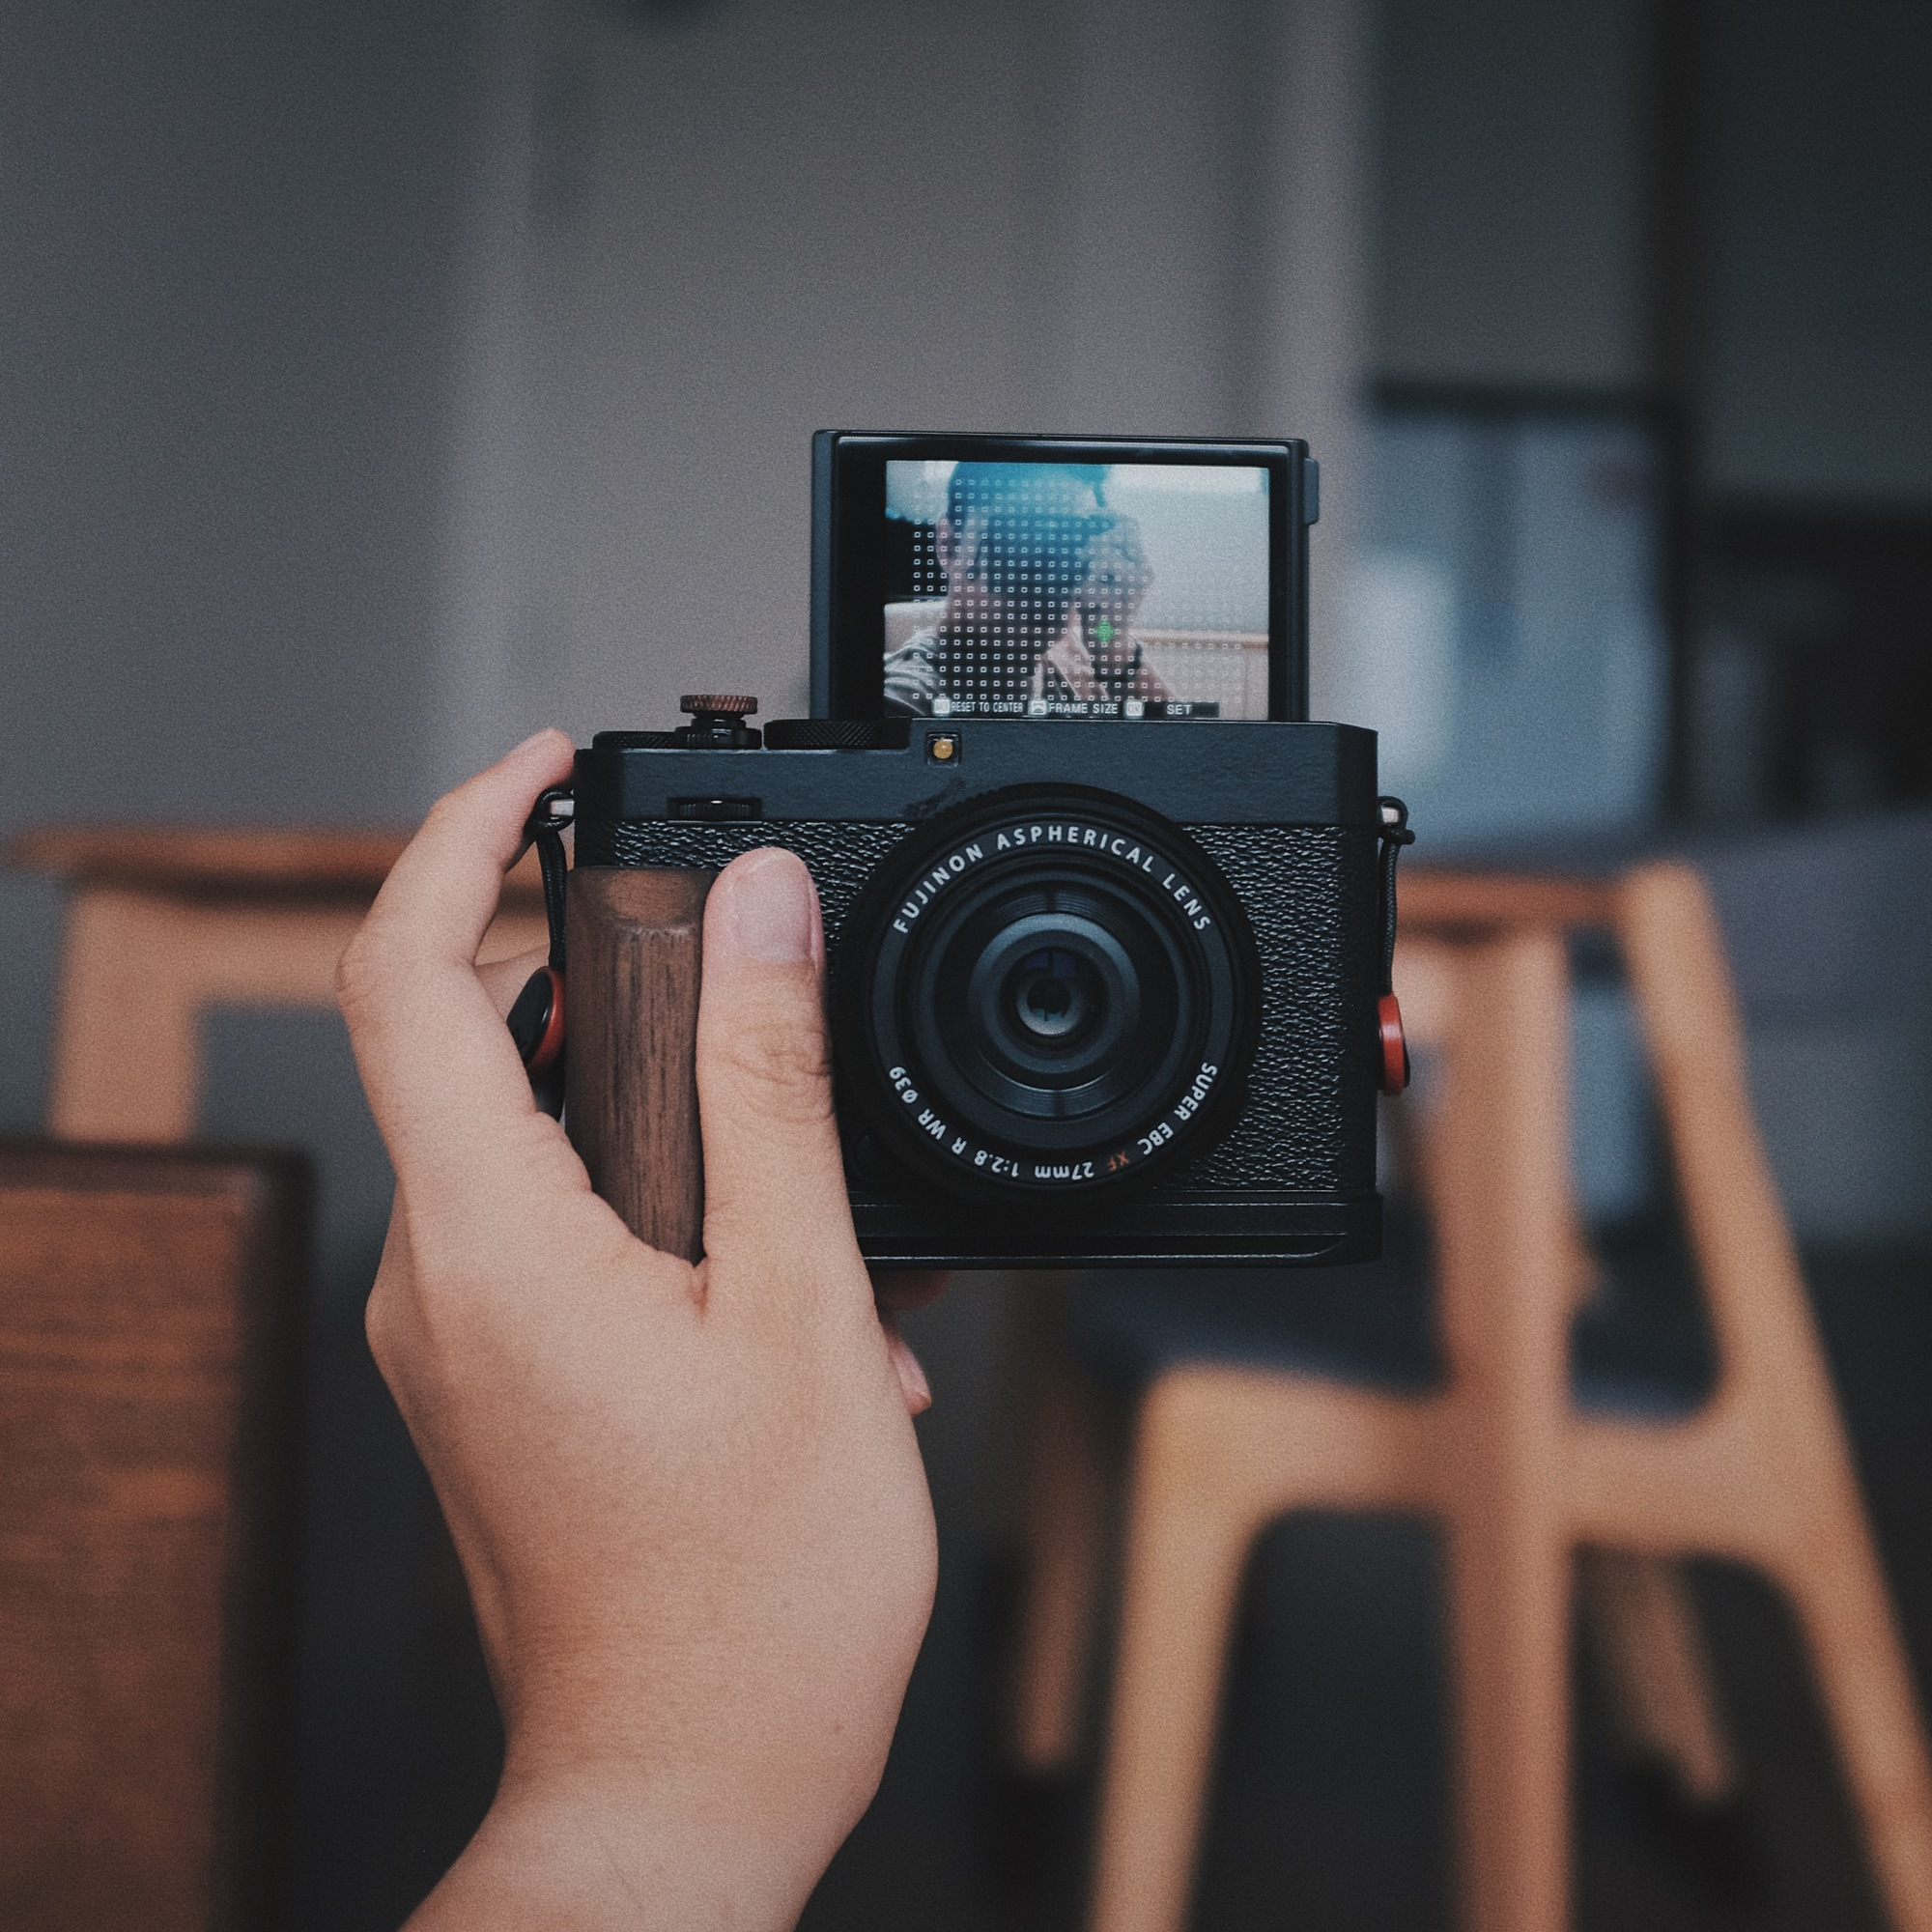
\includegraphics[width=\linewidth]{\envfinaldir/coverpic-prod.jpg}\par
            % \vskip 30pt
            \vfill

            \normalsize\rmfamily\scshape
            \copyright{} The Web Digest Project \hfill\large \envdatestr
        \end{center}
    \end{titlepage}
    % \restoregeometry
}
\newcommand{\simplehref}[1]{%
    \textcolor{blue!80!green}{\href{#1}{#1}}%
}
\renewcommand{\contentsname}{\center\Huge\sffamily\bfseries Contents\par\vskip 20pt}
\newcounter{ipartcounter}
\setcounter{ipartcounter}{0}
\newcommand{\ipart}[1]{
    % \vskip 20pt
    \clearpage
    \stepcounter{ipartcounter}
    \phantomsection
    \addcontentsline{toc}{chapter}{#1}
    % \begin{center}
    %     \Huge
    %     \sffamily\bfseries
    %     #1
    % \end{center}
    % \vskip 20pt plus 7pt
}
\newcounter{ichaptercounter}
\setcounter{ichaptercounter}{0}
\newcommand{\ichapter}[1]{
    % \vskip 20pt
    \clearpage
    \stepcounter{ichaptercounter}
    \phantomsection
    \addcontentsline{toc}{section}{\numberline{\arabic{ichaptercounter}}#1}
    \begin{center}
        \Huge
        \sffamily\bfseries
        #1
    \end{center}
    \vskip 20pt plus 7pt
}
\newcommand{\entrytitlefont}[1]{\subsection*{\raggedright\Large\sffamily\bfseries#1}}
\newcommand{\entryitemGeneric}[2]{
    % argv: title, url
    \parbox{\linewidth}{
        \entrytitlefont{#1}\par\vskip 5pt
        \footnotesize\ttfamily\mdseries
        \simplehref{#2}
    }\vskip 11pt plus 11pt minus 1pt
}
\newcommand{\entryitemGithub}[3]{
    % argv: title, url, desc
    \parbox{\linewidth}{
        \entrytitlefont{#1}\par\vskip 5pt
        \footnotesize\ttfamily\mdseries
        \simplehref{#2}\par\vskip 5pt
        \small\rmfamily\mdseries#3
    }\vskip 11pt plus 11pt minus 1pt
}
\newcommand{\entryitemAp}[3]{
    % argv: title, url, desc
    \parbox{\linewidth}{
        \entrytitlefont{#1}\par\vskip 5pt
        \footnotesize\ttfamily\mdseries
        \simplehref{#2}\par\vskip 5pt
        \small\rmfamily\mdseries#3
    }\vskip 11pt plus 11pt minus 1pt
}
\newcommand{\entryitemHackernews}[3]{
    % argv: title, hnurl, rawurl
    % \parbox{\linewidth}{
    %     \entrytitlefont{#1}\par\vskip 5pt
    %     \footnotesize\ttfamily\mdseries
    %     \simplehref{#3}\par
    %     \textcolor{black!50}{\href{#2}{#2}}
    % }\vskip 11pt plus 11pt minus 1pt
    \begin{minipage}{\linewidth}
            \entrytitlefont{#1}\par\vskip 5pt
            \footnotesize\ttfamily\mdseries
            \simplehref{#3}\par
            \textcolor{black!50}{\href{#2}{#2}}
    \end{minipage}\par\vskip 11pt plus 11pt minus 1pt
}







\begin{document}

\makeheader

\tableofcontents\clearpage




\ipart{Developers}
\ichapter{Hacker News}
\entryitemTwoLinks{Anti-aging breakthrough: Stem cells reverse signs of aging in monkeys}{https://news.ycombinator.com/item?id=45454460}{https://www.nad.com/news/anti-aging-breakthrough-stem-cells-reverse-signs-of-aging-in-monkeys}

\entryitemTwoLinks{OpenAI's H1 2025: \$4.3B in income, \$13.5B in loss}{https://news.ycombinator.com/item?id=45453586}{https://www.techinasia.com/news/openais-revenue-rises-16-to-4-3b-in-h1-2025}

\entryitemTwoLinks{Gemini 3.0 Pro – early tests}{https://news.ycombinator.com/item?id=45453448}{https://twitter.com/chetaslua/status/1973694615518880236}

\entryitemTwoLinks{Babel is why I keep blogging with Emacs}{https://news.ycombinator.com/item?id=45453222}{https://entropicthoughts.com/why-stick-to-emacs-blog}

\entryitemTwoLinks{Email immutability matters more in a world with AI}{https://news.ycombinator.com/item?id=45453135}{https://www.fastmail.com/blog/not-written-with-ai/}

\entryitemTwoLinks{Why I chose Lua for this blog}{https://news.ycombinator.com/item?id=45452261}{https://andregarzia.com/2025/03/why-i-choose-lua-for-this-blog.html}

\entryitemTwoLinks{Playball – Watch MLB games from a terminal}{https://news.ycombinator.com/item?id=45451577}{https://github.com/paaatrick/playball}

\entryitemTwoLinks{Signal Protocol and Post-Quantum Ratchets}{https://news.ycombinator.com/item?id=45451527}{https://signal.org/blog/spqr/}

\entryitemTwoLinks{Windows 7 marketshare jumps to nearly 10\% as Windows 10 support is about to end}{https://news.ycombinator.com/item?id=45451208}{https://www.neowin.net/news/windows-7-marketshare-jumps-to-nearly-10-as-windows-10-enters-final-weeks-of-support/}

\entryitemTwoLinks{Autism should not be seen as single condition with one cause, say scientists}{https://news.ycombinator.com/item?id=45451103}{https://www.theguardian.com/society/2025/oct/01/autism-should-not-be-seen-as-single-condition-with-one-cause-say-scientists}

\entryitemTwoLinks{Work is not school: Surviving institutional stupidity}{https://news.ycombinator.com/item?id=45450525}{https://www.leadingsapiens.com/surviving-institutional-stupidity/}

\entryitemTwoLinks{Two Amazon delivery drones crash into crane in commercial area of Tolleson, AZ}{https://news.ycombinator.com/item?id=45450449}{https://www.abc15.com/news/region-west-valley/tolleson/two-amazon-delivery-drones-crash-into-crane-in-commercial-area-of-tolleson}

\entryitemTwoLinks{N8n added native persistent storage with DataTables}{https://news.ycombinator.com/item?id=45450044}{https://community.n8n.io/t/data-tables-are-here/192256}

\entryitemTwoLinks{Potential issues in curl found using AI assisted tools}{https://news.ycombinator.com/item?id=45449348}{https://mastodon.social/@bagder/115241241075258997}

\entryitemTwoLinks{Meta will listen into AI conversations to personalize ads}{https://news.ycombinator.com/item?id=45448839}{https://www.theregister.com/2025/10/01/meta\_ai\_use\_informs\_ads/}

\entryitemTwoLinks{EU funds are flowing into spyware companies and politicians demanding answers}{https://news.ycombinator.com/item?id=45448825}{https://www.theregister.com/2025/10/02/eu\_spyware\_funding/}

\entryitemTwoLinks{Red Hat confirms security incident after hackers breach GitLab instance}{https://news.ycombinator.com/item?id=45448772}{https://www.bleepingcomputer.com/news/security/red-hat-confirms-security-incident-after-hackers-claim-github-breach/}

\entryitemTwoLinks{NL Judge: Meta must respect user's choice of recommendation system}{https://news.ycombinator.com/item?id=45448326}{https://www.bitsoffreedom.nl/2025/10/02/judge-in-the-bits-of-freedom-vs-meta-lawsuit-meta-must-respect-users-choice/}

\entryitemTwoLinks{How the AI Bubble Will Pop}{https://news.ycombinator.com/item?id=45448199}{https://www.derekthompson.org/p/this-is-how-the-ai-bubble-will-pop}

\entryitemTwoLinks{How Israeli actions caused famine in Gaza, visualized}{https://news.ycombinator.com/item?id=45447699}{https://www.cnn.com/2025/10/02/middleeast/gaza-famine-causes-vis-intl}\ichapter{Phoronix}
\entryitemGeneric{\hskip 0pt{}Linux 6.18 To More Reliably Handle 255+ vCPUs On AMD EPYC Servers}{https://www.phoronix.com/news/Linux-6.18-Better-EPYC-256-vCPU}

\entryitemGeneric{\hskip 0pt{}Linus Torvalds Vents Over "Completely Crazy Rust Format Checking"}{https://www.phoronix.com/news/Linus-Torvalds-Rust-Formatting}

\entryitemGeneric{\hskip 0pt{}ZLUDA 5 Released With An Offline Compiler For CUDA On Non-NVIDIA GPUs}{https://www.phoronix.com/news/ZLUDA-5-Released}

\entryitemGeneric{\hskip 0pt{}SiFive Premier P550, Apple M2 Pro/Max/Ultra DTs \& Other SoC Changes For Linux 6.18}{https://www.phoronix.com/news/Linux-6.18-SoC-DT-Changes}

\entryitemGeneric{\hskip 0pt{}Linux 6.18 Kbuild Brings An Optimization For gen\_init\_cpio On Btrfs Or XFS}{https://www.phoronix.com/news/Linux-6.18-Kbuild}

\entryitemGeneric{\hskip 0pt{}Second Beta Of KDE Plasma 6.5 Released For Testing}{https://www.phoronix.com/news/KDE-Plasma-6.5-Beta-2}

\entryitemGeneric{\hskip 0pt{}Intel Posts Linux Driver Patches For Nova Lake Audio Support}{https://www.phoronix.com/news/Intel-Nova-Lake-Audio-Support}

\entryitemGeneric{\hskip 0pt{}Raspberry Pi OS Updated Against Debian 13 Trixie}{https://www.phoronix.com/news/Raspberry-Pi-OS-Debian-13}

\entryitemGeneric{\hskip 0pt{}Signed Programs \& Other BPF Changes Merged For Linux 6.18}{https://www.phoronix.com/news/Linux--6.18-BPF}


\ipart{Developers~~~~(zh-Hans)}
\ichapter{Solidot}
\entryitemGeneric{\hskip 0pt{}黑客声称入侵了 Red Hat 的 GitHub 代码库}{https://www.solidot.org/story?sid=82469}

\entryitemGeneric{\hskip 0pt{}千禧一代癌症发病率在上升}{https://www.solidot.org/story?sid=82468}

\entryitemGeneric{\hskip 0pt{}城市空气检测出致病性酵母菌株}{https://www.solidot.org/story?sid=82467}

\entryitemGeneric{\hskip 0pt{}珍·古道尔去世,享年 91 岁}{https://www.solidot.org/story?sid=82466}

\entryitemGeneric{\hskip 0pt{}Kindle Scribe 加入 AI 驱动的笔记本功能}{https://www.solidot.org/story?sid=82465}

\entryitemGeneric{\hskip 0pt{}Imgur 屏蔽英国用户访问}{https://www.solidot.org/story?sid=82464}

\entryitemGeneric{\hskip 0pt{}微软宣布 Windows 11 v25H2 GA}{https://www.solidot.org/story?sid=82463}

\entryitemGeneric{\hskip 0pt{}Cloudflare 赞助 Ladybird 浏览器引擎项目}{https://www.solidot.org/story?sid=82462}

\entryitemGeneric{\hskip 0pt{}阿富汗断网超过两天}{https://www.solidot.org/story?sid=82461}

\entryitemGeneric{\hskip 0pt{}Linus Torvalds 从 Linux 6.18 中完全移除了 Bcachefs }{https://www.solidot.org/story?sid=82460}

\entryitemGeneric{\hskip 0pt{}世界最高大桥花江峡谷大桥通车}{https://www.solidot.org/story?sid=82459}

\entryitemGeneric{\hskip 0pt{}CS 教授警告毕业生难找到工作}{https://www.solidot.org/story?sid=82458}

\entryitemGeneric{\hskip 0pt{}因 AI 需求大涨 DRAM 价格翻倍}{https://www.solidot.org/story?sid=82457}

\entryitemGeneric{\hskip 0pt{}微塑料可能削弱骨骼}{https://www.solidot.org/story?sid=82456}\ichapter{V2EX}
\entryitemGeneric{\hskip 0pt{}[macOS] 推荐升级系统}{https://www.v2ex.com/t/1163203}

\entryitemGeneric{\hskip 0pt{}[数据库] 靓仔们, DataGrip 非商用免费了}{https://www.v2ex.com/t/1163202}

\entryitemGeneric{\hskip 0pt{}[美酒与美食] 这些年 我感激的预制菜}{https://www.v2ex.com/t/1163201}

\entryitemGeneric{\hskip 0pt{}[Google] 谷歌 不仅 砍软件 也砍硬件}{https://www.v2ex.com/t/1163200}

\entryitemGeneric{\hskip 0pt{}[分享创造] 假期人太多了,在家玩 sora 2}{https://www.v2ex.com/t/1163199}

\entryitemGeneric{\hskip 0pt{}[分享发现] [悲报]免费的美国手机号码 Helium-Mobile 最新政策,使得要跟白嫖方案 Zero Plan 说再见了}{https://www.v2ex.com/t/1163198}

\entryitemGeneric{\hskip 0pt{}[iPhone] 记录 Apple 逆天 ERS(快速更换服务)使用过程}{https://www.v2ex.com/t/1163196}

\entryitemGeneric{\hskip 0pt{}[开源软件] 撸了 azkaban 中文版,支持中英文切换 开源共享}{https://www.v2ex.com/t/1163194}

\entryitemGeneric{\hskip 0pt{}[分享创造] 我把几乎所有的``nano banana''功能都塞进了这个站 nanobanananano.space}{https://www.v2ex.com/t/1163193}

\entryitemGeneric{\hskip 0pt{}[分享创造] 再嗑一个 AI 图片站,目前我最满意的一个站 搞了 3 周终于上线了}{https://www.v2ex.com/t/1163192}

\entryitemGeneric{\hskip 0pt{}[Android] 安卓 7.1.1 的旧手机,还能装些什么软件吗}{https://www.v2ex.com/t/1163191}

\entryitemGeneric{\hskip 0pt{}[微信] 微信 for Linux 终于更新了}{https://www.v2ex.com/t/1163189}

\entryitemGeneric{\hskip 0pt{}[分享创造] Creat by Jaden@Business, sora 2, Sora 2 is here}{https://www.v2ex.com/t/1163188}

\entryitemGeneric{\hskip 0pt{}[问与答] sora2 需求量大不?}{https://www.v2ex.com/t/1163187}

\entryitemGeneric{\hskip 0pt{}[推广] videosora2.com 上线啦 🎉}{https://www.v2ex.com/t/1163186}

\entryitemGeneric{\hskip 0pt{}[推广] Sidefy - 屏幕边缘信息流 更新了较大版本,增加了之前 v 友提的上边缘停靠需求和不透明模式}{https://www.v2ex.com/t/1163185}

\entryitemGeneric{\hskip 0pt{}[分享创造] 2025 年, Java 是最适合的脚本语言:用 AI 写 100 个 Java 小应用}{https://www.v2ex.com/t/1163183}

\entryitemGeneric{\hskip 0pt{}[游戏] 怎么样才能找到更多可以 iframe 的游戏网站呢?}{https://www.v2ex.com/t/1163180}

\entryitemGeneric{\hskip 0pt{}[Python] fastapi-router-viz, 可视化你的 API 内依赖关系}{https://www.v2ex.com/t/1163179}

\entryitemGeneric{\hskip 0pt{}[iPhone] 移动电信双卡用 iPhone 有什么好办法吗?}{https://www.v2ex.com/t/1163177}

\entryitemGeneric{\hskip 0pt{}[分享发现] 如果你的电脑有前置摄像头,这里有一个有趣的头部追踪 tech demo}{https://www.v2ex.com/t/1163175}

\entryitemGeneric{\hskip 0pt{}[生活] 隔壁有关鸡蛋灌饼的帖子标题不太合适,不该强调预制应该强调难吃}{https://www.v2ex.com/t/1163174}

\entryitemGeneric{\hskip 0pt{}[macOS] 问下大家, m1 有更新 macos26 的吗,可以讲下使用体验吗}{https://www.v2ex.com/t/1163173}

\entryitemGeneric{\hskip 0pt{}[VXNA] 申请移出 VXNA}{https://www.v2ex.com/t/1163172}

\entryitemGeneric{\hskip 0pt{}[问与答] 自建的 vaultwarden 是不是不支持币安身份验证器绑定?}{https://www.v2ex.com/t/1163171}

\entryitemGeneric{\hskip 0pt{}[问与答] 电信宽带总是访问到联通的服务器}{https://www.v2ex.com/t/1163170}

\entryitemGeneric{\hskip 0pt{}[健康] 脑洞大开:颈椎病是不是由于移动互联网带来的?}{https://www.v2ex.com/t/1163167}

\entryitemGeneric{\hskip 0pt{}[酷工作] 上海外企甲方招聘: SAP Security / GRC Lead, 40W+}{https://www.v2ex.com/t/1163165}

\entryitemGeneric{\hskip 0pt{}[电动汽车] 想买一辆二手的特斯拉,请教一下各位哪个渠道比较好?}{https://www.v2ex.com/t/1163162}

\entryitemGeneric{\hskip 0pt{}[Claude] 用了半个月 Claude code 200max ,突然全款给我退了,这是为什么?}{https://www.v2ex.com/t/1163161}

\entryitemGeneric{\hskip 0pt{}[macOS] MacOS 能自定义触发角来运行第三方应用吗}{https://www.v2ex.com/t/1163160}

\entryitemGeneric{\hskip 0pt{}[Solana] 十月暴涨已经开始了,财富自由的机会就在未来一百天}{https://www.v2ex.com/t/1163159}

\entryitemGeneric{\hskip 0pt{}[阅读] [记录]-2025-10-02 最近在读的书}{https://www.v2ex.com/t/1163158}

\entryitemGeneric{\hskip 0pt{}[问与答] V2EX 是禁止 copilot(AI)抓取页面了吗?}{https://www.v2ex.com/t/1163157}

\entryitemGeneric{\hskip 0pt{}[问与答] 求一刀代付卡的网站}{https://www.v2ex.com/t/1163156}

\entryitemGeneric{\hskip 0pt{}[Apple] 国区 Apple 🆔设备成功购买 Apple care one 的折腾全过程。}{https://www.v2ex.com/t/1163155}

\entryitemGeneric{\hskip 0pt{}[音乐] 女儿最近经常自己即兴编一些歌,大佬们有什么简单傻瓜式的 AI 编曲方案?}{https://www.v2ex.com/t/1163151}

\entryitemGeneric{\hskip 0pt{}[问与答] 有可以玩游戏的虚拟机程序吗?}{https://www.v2ex.com/t/1163149}

\entryitemGeneric{\hskip 0pt{}[Telegram] Telegram 频道精华贴检索机器人}{https://www.v2ex.com/t/1163148}

\entryitemGeneric{\hskip 0pt{}[推广] videosora2.com 发布啦~}{https://www.v2ex.com/t/1163146}

\entryitemGeneric{\hskip 0pt{}[问与答] Hubstudio 更新到 V3.46.0 (64) 后,某些站提示``无法访问此网站'',该怎么解决?}{https://www.v2ex.com/t/1163145}

\entryitemGeneric{\hskip 0pt{}[程序员] 在纠结玩玩 CodeX 和 ClaudeCode, CodeX 使用需要开全局吗}{https://www.v2ex.com/t/1163144}

\entryitemGeneric{\hskip 0pt{}[NAS] 腾讯极光 5s 盒子如何开启 ssh}{https://www.v2ex.com/t/1163143}

\entryitemGeneric{\hskip 0pt{}[程序员] 狠狠共情啥叫"窃取革命胜利果实"这话. 我的 nyt pips game 游戏,被老登整站复制😡}{https://www.v2ex.com/t/1163141}

\entryitemGeneric{\hskip 0pt{}[分享发现] AI Detector - 图片检测}{https://www.v2ex.com/t/1163140}

\entryitemGeneric{\hskip 0pt{}[程序员] Claude 4.5 (feat: claude desktop), 一款最像人的 AI: In a bad way}{https://www.v2ex.com/t/1163138}

\entryitemGeneric{\hskip 0pt{}[Surge] surge for Mac 出现这个提示怎么破?}{https://www.v2ex.com/t/1163137}

\entryitemGeneric{\hskip 0pt{}[问与答] PosterMapsPro - City Map Art Poster Customization Tool}{https://www.v2ex.com/t/1163136}

\entryitemGeneric{\hskip 0pt{}[机械键盘] 可以放在 MacBook pro 键盘区的机械键盘有何推荐 最好是便携一些的}{https://www.v2ex.com/t/1163135}

\entryitemGeneric{\hskip 0pt{}[OpenAI] openrouter 国内访问稳定吗}{https://www.v2ex.com/t/1163133}


\ipart{Generic News}







\clearpage
\leavevmode\vfill
\footnotesize

Copyright \copyright{} 2023-2025 Neruthes and other contributors.

This document is published with CC BY-NC-ND 4.0 license.

The entries listed in this newsletter may be copyrighted by their respective creators.

This newsletter is generated by the Web Digest project.

The newsletters are also delivered via Telegram channel \CJKunderline{\href{https://t.me/webdigestchannel}{https://t.me/webdigestchannel}}.\\
RSS feed is available at \CJKunderline{\href{https://webdigest.pages.dev/rss.xml}{https://webdigest.pages.dev/rss.xml}}.

This newsletter is available in PDF at
\CJKunderline{\href{https://webdigest.pages.dev/}{https://webdigest.pages.dev/}}.

The source code being used to generate this newsletter is available at\\
\CJKunderline{\href{https://github.com/neruthes/webdigest}{https://github.com/neruthes/webdigest}}.

This newsletter is also available in
\CJKunderline{\href{http://webdigest.pages.dev/readhtml/\envyear/WebDigest-20251003.html}{HTML}} and
\CJKunderline{\href{https://github.com/neruthes/webdigest/blob/master/markdown/\envyear/WebDigest-20251003.md}{Markdown}}.


\coverpic{https://unsplash.com/photos/woman-walking-on-a-wet-street-at-night-XkiX71CJxe4}{Julio Lopez}


\end{document}
